\documentclass[1p]{elsarticle_modified}
%\bibliographystyle{elsarticle-num}

%\usepackage[colorlinks]{hyperref}
%\usepackage{abbrmath_seonhwa} %\Abb, \Ascr, \Acal ,\Abf, \Afrak
\usepackage{amsfonts}
\usepackage{amssymb}
\usepackage{amsmath}
\usepackage{amsthm}
\usepackage{scalefnt}
\usepackage{amsbsy}
\usepackage{kotex}
\usepackage{caption}
\usepackage{subfig}
\usepackage{color}
\usepackage{graphicx}
\usepackage{xcolor} %% white, black, red, green, blue, cyan, magenta, yellow
\usepackage{float}
\usepackage{setspace}
\usepackage{hyperref}

\usepackage{tikz}
\usetikzlibrary{arrows}

\usepackage{multirow}
\usepackage{array} % fixed length table
\usepackage{hhline}

%%%%%%%%%%%%%%%%%%%%%
\makeatletter
\renewcommand*\env@matrix[1][\arraystretch]{%
	\edef\arraystretch{#1}%
	\hskip -\arraycolsep
	\let\@ifnextchar\new@ifnextchar
	\array{*\c@MaxMatrixCols c}}
\makeatother %https://tex.stackexchange.com/questions/14071/how-can-i-increase-the-line-spacing-in-a-matrix
%%%%%%%%%%%%%%%

\usepackage[normalem]{ulem}

\newcommand{\msout}[1]{\ifmmode\text{\sout{\ensuremath{#1}}}\else\sout{#1}\fi}
%SOURCE: \msout is \stkout macro in https://tex.stackexchange.com/questions/20609/strikeout-in-math-mode

\newcommand{\cancel}[1]{
	\ifmmode
	{\color{red}\msout{#1}}
	\else
	{\color{red}\sout{#1}}
	\fi
}

\newcommand{\add}[1]{
	{\color{blue}\uwave{#1}}
}

\newcommand{\replace}[2]{
	\ifmmode
	{\color{red}\msout{#1}}{\color{blue}\uwave{#2}}
	\else
	{\color{red}\sout{#1}}{\color{blue}\uwave{#2}}
	\fi
}

\newcommand{\Sol}{\mathcal{S}} %segment
\newcommand{\D}{D} %diagram
\newcommand{\A}{\mathcal{A}} %arc


%%%%%%%%%%%%%%%%%%%%%%%%%%%%%5 test

\def\sl{\operatorname{\textup{SL}}(2,\Cbb)}
\def\psl{\operatorname{\textup{PSL}}(2,\Cbb)}
\def\quan{\mkern 1mu \triangleright \mkern 1mu}

\theoremstyle{definition}
\newtheorem{thm}{Theorem}[section]
\newtheorem{prop}[thm]{Proposition}
\newtheorem{lem}[thm]{Lemma}
\newtheorem{ques}[thm]{Question}
\newtheorem{cor}[thm]{Corollary}
\newtheorem{defn}[thm]{Definition}
\newtheorem{exam}[thm]{Example}
\newtheorem{rmk}[thm]{Remark}
\newtheorem{alg}[thm]{Algorithm}

\newcommand{\I}{\sqrt{-1}}
\begin{document}

%\begin{frontmatter}
%
%\title{Boundary parabolic representations of knots up to 8 crossings}
%
%%% Group authors per affiliation:
%\author{Yunhi Cho} 
%\address{Department of Mathematics, University of Seoul, Seoul, Korea}
%\ead{yhcho@uos.ac.kr}
%
%
%\author{Seonhwa Kim} %\fnref{s_kim}}
%\address{Center for Geometry and Physics, Institute for Basic Science, Pohang, 37673, Korea}
%\ead{ryeona17@ibs.re.kr}
%
%\author{Hyuk Kim}
%\address{Department of Mathematical Sciences, Seoul National University, Seoul 08826, Korea}
%\ead{hyukkim@snu.ac.kr}
%
%\author{Seokbeom Yoon}
%\address{Department of Mathematical Sciences, Seoul National University, Seoul, 08826,  Korea}
%\ead{sbyoon15@snu.ac.kr}
%
%\begin{abstract}
%We find all boundary parabolic representation of knots up to 8 crossings.
%
%\end{abstract}
%\begin{keyword}
%    \MSC[2010] 57M25 
%\end{keyword}
%
%\end{frontmatter}

%\linenumbers
%\tableofcontents
%
\newcommand\colored[1]{\textcolor{white}{\rule[-0.35ex]{0.8em}{1.4ex}}\kern-0.8em\color{red} #1}%
%\newcommand\colored[1]{\textcolor{white}{ #1}\kern-2.17ex	\textcolor{white}{ #1}\kern-1.81ex	\textcolor{white}{ #1}\kern-2.15ex\color{red}#1	}

{\Large $\underline{11n_{11}~(K11n_{11})}$}

\setlength{\tabcolsep}{10pt}
\renewcommand{\arraystretch}{1.6}
\vspace{1cm}\begin{tabular}{m{100pt}>{\centering\arraybackslash}m{274pt}}
\multirow{5}{120pt}{
	\centering
	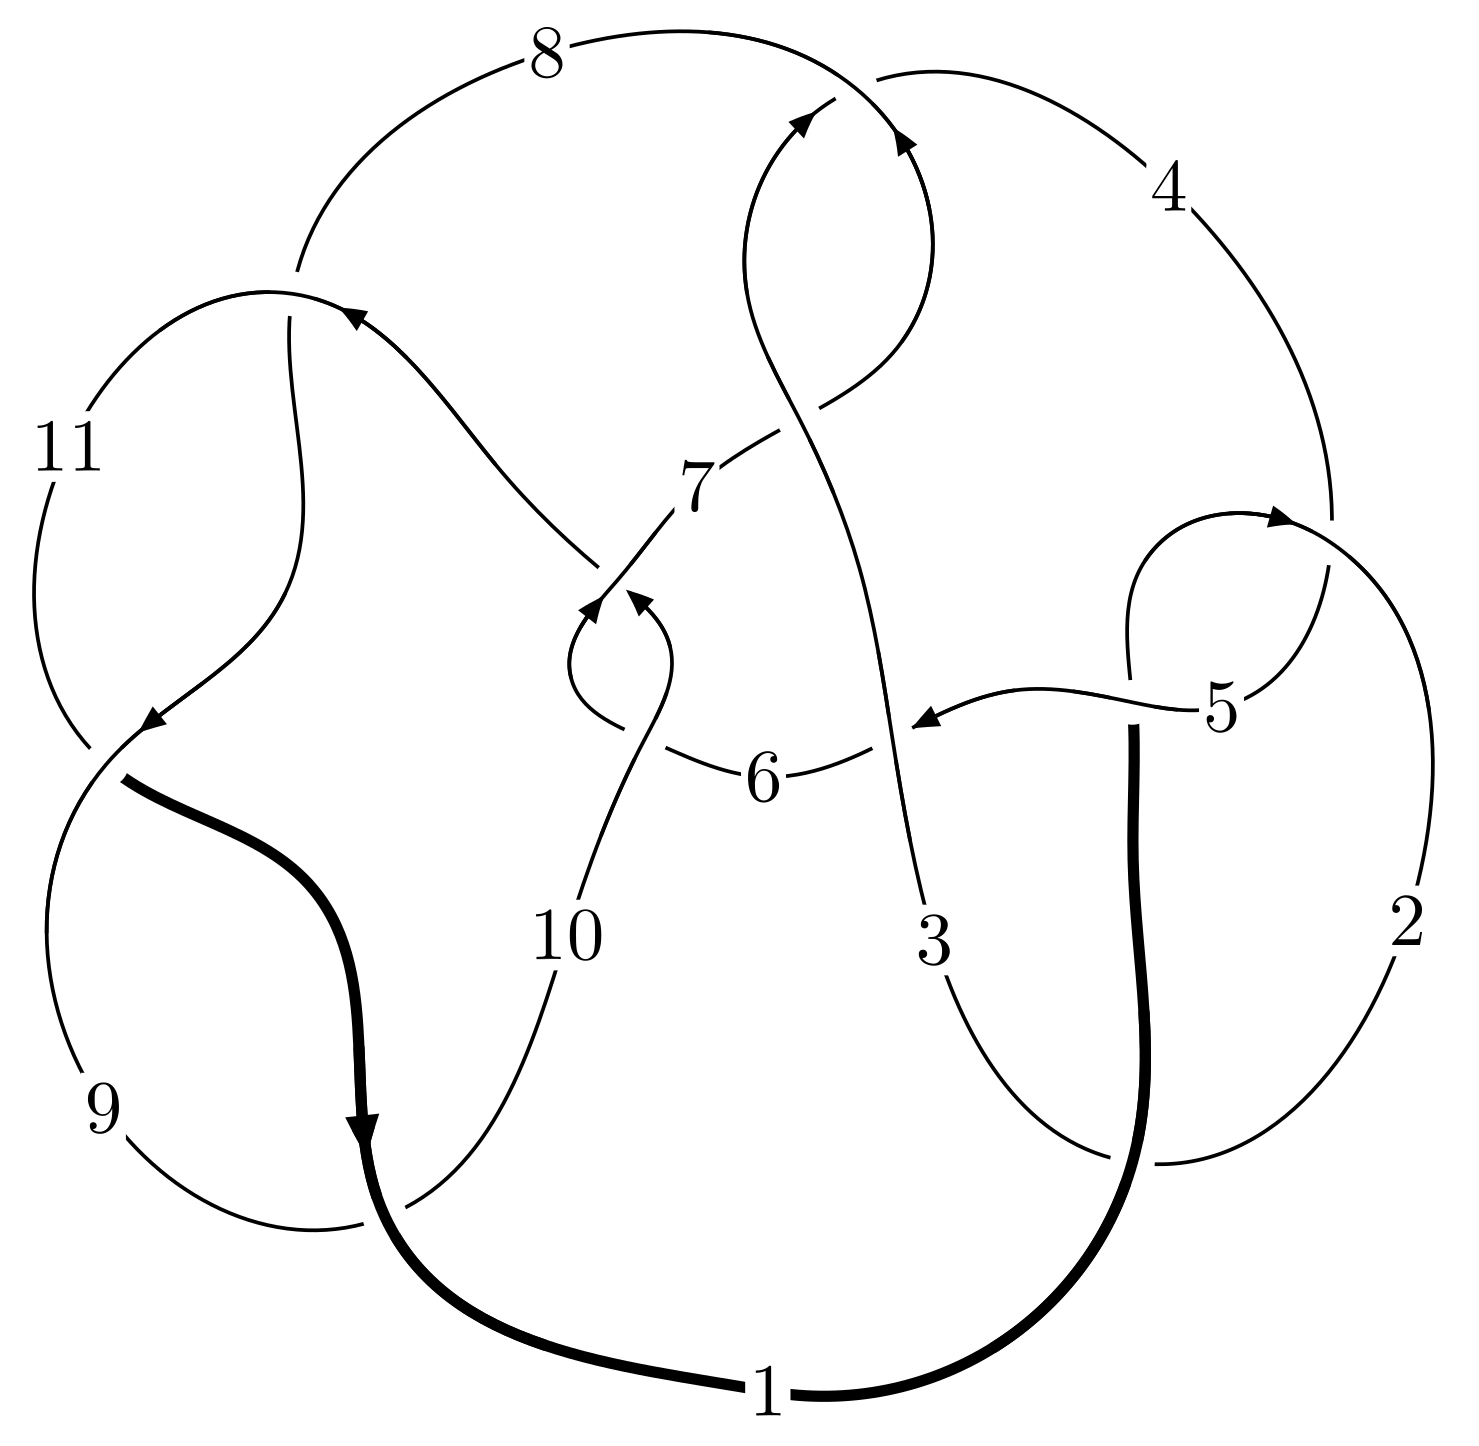
\includegraphics[width=112pt]{../../../GIT/diagram.site/Diagrams/png/627_11n_11.png}\\
\ \ \ A knot diagram\footnotemark}&
\allowdisplaybreaks
\textbf{Linearized knot diagam} \\
\cline{2-2}
 &
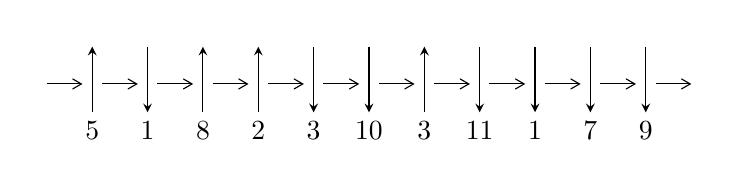
\begin{tikzpicture}[x=20pt, y=17pt]
	% nodes
	\node (C0) at (0, 0) {};
	\node (C1) at (1, 0) {};
	\node (C1U) at (1, +1) {};
	\node (C1D) at (1, -1) {5};

	\node (C2) at (2, 0) {};
	\node (C2U) at (2, +1) {};
	\node (C2D) at (2, -1) {1};

	\node (C3) at (3, 0) {};
	\node (C3U) at (3, +1) {};
	\node (C3D) at (3, -1) {8};

	\node (C4) at (4, 0) {};
	\node (C4U) at (4, +1) {};
	\node (C4D) at (4, -1) {2};

	\node (C5) at (5, 0) {};
	\node (C5U) at (5, +1) {};
	\node (C5D) at (5, -1) {3};

	\node (C6) at (6, 0) {};
	\node (C6U) at (6, +1) {};
	\node (C6D) at (6, -1) {10};

	\node (C7) at (7, 0) {};
	\node (C7U) at (7, +1) {};
	\node (C7D) at (7, -1) {3};

	\node (C8) at (8, 0) {};
	\node (C8U) at (8, +1) {};
	\node (C8D) at (8, -1) {11};

	\node (C9) at (9, 0) {};
	\node (C9U) at (9, +1) {};
	\node (C9D) at (9, -1) {1};

	\node (C10) at (10, 0) {};
	\node (C10U) at (10, +1) {};
	\node (C10D) at (10, -1) {7};

	\node (C11) at (11, 0) {};
	\node (C11U) at (11, +1) {};
	\node (C11D) at (11, -1) {9};
	\node (C12) at (12, 0) {};

	% arrows
	\draw[->,>={angle 60}]
	(C0) edge (C1) (C1) edge (C2) (C2) edge (C3) (C3) edge (C4) (C4) edge (C5) (C5) edge (C6) (C6) edge (C7) (C7) edge (C8) (C8) edge (C9) (C9) edge (C10) (C10) edge (C11) (C11) edge (C12) ;	\draw[->,>=stealth]
	(C1D) edge (C1U) (C2U) edge (C2D) (C3D) edge (C3U) (C4D) edge (C4U) (C5U) edge (C5D) (C6U) edge (C6D) (C7D) edge (C7U) (C8U) edge (C8D) (C9U) edge (C9D) (C10U) edge (C10D) (C11U) edge (C11D) ;
	\end{tikzpicture} \\
\hhline{~~} \\& 
\textbf{Solving Sequence} \\ \cline{2-2} 
 &
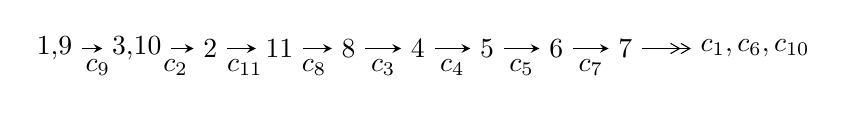
\begin{tikzpicture}[x=25pt, y=7pt]
	% node
	\node (A0) at (-1/8, 0) {1,9};
	\node (A1) at (17/16, 0) {3,10};
	\node (A2) at (17/8, 0) {2};
	\node (A3) at (25/8, 0) {11};
	\node (A4) at (33/8, 0) {8};
	\node (A5) at (41/8, 0) {4};
	\node (A6) at (49/8, 0) {5};
	\node (A7) at (57/8, 0) {6};
	\node (A8) at (65/8, 0) {7};
	\node (C1) at (1/2, -1) {$c_{9}$};
	\node (C2) at (13/8, -1) {$c_{2}$};
	\node (C3) at (21/8, -1) {$c_{11}$};
	\node (C4) at (29/8, -1) {$c_{8}$};
	\node (C5) at (37/8, -1) {$c_{3}$};
	\node (C6) at (45/8, -1) {$c_{4}$};
	\node (C7) at (53/8, -1) {$c_{5}$};
	\node (C8) at (61/8, -1) {$c_{7}$};
	\node (A9) at (10, 0) {$c_{1},c_{6},c_{10}$};

	% edge
	\draw[->,>=stealth]	
	(A0) edge (A1) (A1) edge (A2) (A2) edge (A3) (A3) edge (A4) (A4) edge (A5) (A5) edge (A6) (A6) edge (A7) (A7) edge (A8) ;
	\draw[->>,>={angle 60}]	
	(A8) edge (A9);
\end{tikzpicture} \\ 

\end{tabular} \\

\footnotetext{
The image of knot diagram is generated by the software ``\textbf{Draw programme}" developed by Andrew Bartholomew(\url{http://www.layer8.co.uk/maths/draw/index.htm\#Running-draw}), where we modified some parts for our purpose(\url{https://github.com/CATsTAILs/LinksPainter}).
}\phantom \\ \newline 
\centering \textbf{Ideals for irreducible components\footnotemark of $X_{\text{par}}$} 
 
\begin{align*}
I^u_{1}&=\langle 
-1.47912\times10^{16} u^{30}-9.15523\times10^{16} u^{29}+\cdots+4.49053\times10^{16} b-7.04624\times10^{16},\\
\phantom{I^u_{1}}&\phantom{= \langle  }9.09026\times10^{16} u^{30}+2.68470\times10^{17} u^{29}+\cdots+8.98106\times10^{16} a-6.04967\times10^{16},\;u^{31}+3 u^{30}+\cdots-2 u-1\rangle \\
I^u_{2}&=\langle 
a u+b,\;a^2+a u+a+u+2,\;u^2+u-1\rangle \\
\\
\end{align*}
\raggedright * 2 irreducible components of $\dim_{\mathbb{C}}=0$, with total 35 representations.\\
\footnotetext{All coefficients of polynomials are rational numbers. But the coefficients are sometimes approximated in decimal forms when there is not enough margin.}
\newpage
\renewcommand{\arraystretch}{1}
\centering \section*{I. $I^u_{1}= \langle -1.48\times10^{16} u^{30}-9.16\times10^{16} u^{29}+\cdots+4.49\times10^{16} b-7.05\times10^{16},\;9.09\times10^{16} u^{30}+2.68\times10^{17} u^{29}+\cdots+8.98\times10^{16} a-6.05\times10^{16},\;u^{31}+3 u^{30}+\cdots-2 u-1 \rangle$}
\flushleft \textbf{(i) Arc colorings}\\
\begin{tabular}{m{7pt} m{180pt} m{7pt} m{180pt} }
\flushright $a_{1}=$&$\begin{pmatrix}0\\u\end{pmatrix}$ \\
\flushright $a_{9}=$&$\begin{pmatrix}1\\0\end{pmatrix}$ \\
\flushright $a_{3}=$&$\begin{pmatrix}-1.01216 u^{30}-2.98929 u^{29}+\cdots+1.56951 u+0.673603\\0.329386 u^{30}+2.03879 u^{29}+\cdots+4.20243 u+1.56913\end{pmatrix}$ \\
\flushright $a_{10}=$&$\begin{pmatrix}1\\u^2\end{pmatrix}$ \\
\flushright $a_{2}=$&$\begin{pmatrix}-1.01216 u^{30}-2.98929 u^{29}+\cdots+1.56951 u+0.673603\\0.286170 u^{30}+2.18539 u^{29}+\cdots+5.12021 u+1.52195\end{pmatrix}$ \\
\flushright $a_{11}=$&$\begin{pmatrix}u\\u\end{pmatrix}$ \\
\flushright $a_{8}=$&$\begin{pmatrix}- u^2+1\\- u^2\end{pmatrix}$ \\
\flushright $a_{4}=$&$\begin{pmatrix}-1.10717 u^{30}-3.23912 u^{29}+\cdots+2.61916 u+1.31094\\0.286732 u^{30}+2.01767 u^{29}+\cdots+4.39808 u+1.64078\end{pmatrix}$ \\
\flushright $a_{5}=$&$\begin{pmatrix}-0.337359 u^{30}-1.17932 u^{29}+\cdots-1.54516 u-1.51176\\0.771351 u^{30}+3.37765 u^{29}+\cdots+4.57039 u+1.23084\end{pmatrix}$ \\
\flushright $a_{6}=$&$\begin{pmatrix}0.366419 u^{30}+0.837409 u^{29}+\cdots-2.16675 u+1.16374\\0.563901 u^{30}+2.05823 u^{29}+\cdots-0.204628 u+0.0803200\end{pmatrix}$ \\
\flushright $a_{7}=$&$\begin{pmatrix}0.0898867 u^{30}+0.521942 u^{29}+\cdots+2.11940 u-0.821574\\-0.252282 u^{30}-0.960869 u^{29}+\cdots+0.641800 u-0.0898867\end{pmatrix}$\\ \flushright $a_{7}=$&$\begin{pmatrix}0.0898867 u^{30}+0.521942 u^{29}+\cdots+2.11940 u-0.821574\\-0.252282 u^{30}-0.960869 u^{29}+\cdots+0.641800 u-0.0898867\end{pmatrix}$\\&\end{tabular}
\flushleft \textbf{(ii) Obstruction class $= -1$}\\~\\
\flushleft \textbf{(iii) Cusp Shapes $= \frac{395916855656835617}{89810629950487196} u^{30}+\frac{295100668624657463}{22452657487621799} u^{29}+\cdots+\frac{1130836942834652079}{89810629950487196} u+\frac{259777290233574227}{44905314975243598}$}\\~\\
\newpage\renewcommand{\arraystretch}{1}
\flushleft \textbf{(iv) u-Polynomials at the component}\newline \\
\begin{tabular}{m{50pt}|m{274pt}}
Crossings & \hspace{64pt}u-Polynomials at each crossing \\
\hline $$\begin{aligned}c_{1},c_{4}\end{aligned}$$&$\begin{aligned}
&u^{31}+3 u^{30}+\cdots+8 u-1
\end{aligned}$\\
\hline $$\begin{aligned}c_{2}\end{aligned}$$&$\begin{aligned}
&u^{31}+9 u^{30}+\cdots+60 u-1
\end{aligned}$\\
\hline $$\begin{aligned}c_{3},c_{7}\end{aligned}$$&$\begin{aligned}
&u^{31}+3 u^{30}+\cdots+112 u+16
\end{aligned}$\\
\hline $$\begin{aligned}c_{5}\end{aligned}$$&$\begin{aligned}
&u^{31}-3 u^{30}+\cdots+4454 u-977
\end{aligned}$\\
\hline $$\begin{aligned}c_{6},c_{10}\end{aligned}$$&$\begin{aligned}
&u^{31}+3 u^{30}+\cdots-2 u^2+1
\end{aligned}$\\
\hline $$\begin{aligned}c_{8},c_{9},c_{11}\end{aligned}$$&$\begin{aligned}
&u^{31}-3 u^{30}+\cdots-2 u+1
\end{aligned}$\\
\hline
\end{tabular}\\~\\
\newpage\renewcommand{\arraystretch}{1}
\flushleft \textbf{(v) Riley Polynomials at the component}\newline \\
\begin{tabular}{m{50pt}|m{274pt}}
Crossings & \hspace{64pt}Riley Polynomials at each crossing \\
\hline $$\begin{aligned}c_{1},c_{4}\end{aligned}$$&$\begin{aligned}
&y^{31}+9 y^{30}+\cdots+60 y-1
\end{aligned}$\\
\hline $$\begin{aligned}c_{2}\end{aligned}$$&$\begin{aligned}
&y^{31}+29 y^{30}+\cdots+5084 y-1
\end{aligned}$\\
\hline $$\begin{aligned}c_{3},c_{7}\end{aligned}$$&$\begin{aligned}
&y^{31}-25 y^{30}+\cdots+1152 y-256
\end{aligned}$\\
\hline $$\begin{aligned}c_{5}\end{aligned}$$&$\begin{aligned}
&y^{31}+49 y^{30}+\cdots+44552308 y-954529
\end{aligned}$\\
\hline $$\begin{aligned}c_{6},c_{10}\end{aligned}$$&$\begin{aligned}
&y^{31}-3 y^{30}+\cdots+4 y-1
\end{aligned}$\\
\hline $$\begin{aligned}c_{8},c_{9},c_{11}\end{aligned}$$&$\begin{aligned}
&y^{31}-23 y^{30}+\cdots+4 y-1
\end{aligned}$\\
\hline
\end{tabular}\\~\\
\newpage\flushleft \textbf{(vi) Complex Volumes and Cusp Shapes}
$$\begin{array}{c|c|c}  
\text{Solutions to }I^u_{1}& \I (\text{vol} + \sqrt{-1}CS) & \text{Cusp shape}\\
 \hline 
\begin{aligned}
u &= -0.931324 + 0.285581 I \\
a &= \phantom{-}0.99198 - 1.54847 I \\
b &= \phantom{-}0.81708 - 1.15583 I\end{aligned}
 & \phantom{-}0.02246 + 4.44381 I & -1.53825 - 8.61147 I \\ \hline\begin{aligned}
u &= -0.931324 - 0.285581 I \\
a &= \phantom{-}0.99198 + 1.54847 I \\
b &= \phantom{-}0.81708 + 1.15583 I\end{aligned}
 & \phantom{-}0.02246 - 4.44381 I & -1.53825 + 8.61147 I \\ \hline\begin{aligned}
u &= -0.094951 + 1.070970 I \\
a &= \phantom{-}1.345330 - 0.258911 I \\
b &= \phantom{-}0.0113180 + 0.1250270 I\end{aligned}
 & \phantom{-}7.95570 - 0.85651 I & \phantom{-}0.056335 - 0.135364 I \\ \hline\begin{aligned}
u &= -0.094951 - 1.070970 I \\
a &= \phantom{-}1.345330 + 0.258911 I \\
b &= \phantom{-}0.0113180 - 0.1250270 I\end{aligned}
 & \phantom{-}7.95570 + 0.85651 I & \phantom{-}0.056335 + 0.135364 I \\ \hline\begin{aligned}
u &= \phantom{-}0.912773 + 0.075536 I \\
a &= -0.542493 - 0.971836 I \\
b &= -0.20963 + 2.46157 I\end{aligned}
 & -1.30863 - 2.18648 I & -32.4747 - 4.2586 I \\ \hline\begin{aligned}
u &= \phantom{-}0.912773 - 0.075536 I \\
a &= -0.542493 + 0.971836 I \\
b &= -0.20963 - 2.46157 I\end{aligned}
 & -1.30863 + 2.18648 I & -32.4747 + 4.2586 I \\ \hline\begin{aligned}
u &= \phantom{-}0.039656 + 1.102600 I \\
a &= -1.49064 + 0.23083 I \\
b &= -0.1140800 - 0.0213786 I\end{aligned}
 & \phantom{-}7.38206 - 7.22461 I & -1.02588 + 4.93399 I \\ \hline\begin{aligned}
u &= \phantom{-}0.039656 - 1.102600 I \\
a &= -1.49064 - 0.23083 I \\
b &= -0.1140800 + 0.0213786 I\end{aligned}
 & \phantom{-}7.38206 + 7.22461 I & -1.02588 - 4.93399 I \\ \hline\begin{aligned}
u &= \phantom{-}1.193910 + 0.091335 I \\
a &= -0.565824 - 0.262901 I \\
b &= -1.10325 - 1.58386 I\end{aligned}
 & -2.79337 - 1.66318 I & -5.72575 + 2.19283 I \\ \hline\begin{aligned}
u &= \phantom{-}1.193910 - 0.091335 I \\
a &= -0.565824 + 0.262901 I \\
b &= -1.10325 + 1.58386 I\end{aligned}
 & -2.79337 + 1.66318 I & -5.72575 - 2.19283 I\\
 \hline 
 \end{array}$$\newpage$$\begin{array}{c|c|c}  
\text{Solutions to }I^u_{1}& \I (\text{vol} + \sqrt{-1}CS) & \text{Cusp shape}\\
 \hline 
\begin{aligned}
u &= -1.168090 + 0.283606 I \\
a &= \phantom{-}1.41177 - 0.15034 I \\
b &= \phantom{-}2.29367 - 0.71716 I\end{aligned}
 & -4.01618 + 5.37811 I & -8.38800 - 7.62748 I \\ \hline\begin{aligned}
u &= -1.168090 - 0.283606 I \\
a &= \phantom{-}1.41177 + 0.15034 I \\
b &= \phantom{-}2.29367 + 0.71716 I\end{aligned}
 & -4.01618 - 5.37811 I & -8.38800 + 7.62748 I \\ \hline\begin{aligned}
u &= \phantom{-}0.779230\phantom{ +0.000000I} \\
a &= \phantom{-}0.0180125\phantom{ +0.000000I} \\
b &= \phantom{-}0.854641\phantom{ +0.000000I}\end{aligned}
 & -1.12597\phantom{ +0.000000I} & -9.35890\phantom{ +0.000000I} \\ \hline\begin{aligned}
u &= \phantom{-}0.623364 + 0.404541 I \\
a &= -0.331674 + 0.339809 I \\
b &= \phantom{-}0.348918 + 0.935748 I\end{aligned}
 & -1.47821 - 0.10102 I & -8.24537 + 0.31125 I \\ \hline\begin{aligned}
u &= \phantom{-}0.623364 - 0.404541 I \\
a &= -0.331674 - 0.339809 I \\
b &= \phantom{-}0.348918 - 0.935748 I\end{aligned}
 & -1.47821 + 0.10102 I & -8.24537 - 0.31125 I \\ \hline\begin{aligned}
u &= -0.679882 + 0.287551 I \\
a &= -0.567508 - 1.103750 I \\
b &= -1.142870 - 0.115620 I\end{aligned}
 & \phantom{-}1.58742 + 1.54591 I & \phantom{-}2.94722 - 4.18501 I \\ \hline\begin{aligned}
u &= -0.679882 - 0.287551 I \\
a &= -0.567508 + 1.103750 I \\
b &= -1.142870 + 0.115620 I\end{aligned}
 & \phantom{-}1.58742 - 1.54591 I & \phantom{-}2.94722 + 4.18501 I \\ \hline\begin{aligned}
u &= -1.287250 + 0.574250 I \\
a &= -0.687751 + 0.701116 I \\
b &= -1.54338 + 1.46018 I\end{aligned}
 & \phantom{-}4.28029 + 6.65397 I & -2.65676 - 3.57953 I \\ \hline\begin{aligned}
u &= -1.287250 - 0.574250 I \\
a &= -0.687751 - 0.701116 I \\
b &= -1.54338 - 1.46018 I\end{aligned}
 & \phantom{-}4.28029 - 6.65397 I & -2.65676 + 3.57953 I \\ \hline\begin{aligned}
u &= \phantom{-}1.33715 + 0.61035 I \\
a &= \phantom{-}0.347578 + 0.887087 I \\
b &= \phantom{-}0.72674 + 1.60463 I\end{aligned}
 & \phantom{-}3.39903 + 1.19447 I & -2.39419 - 1.64836 I\\
 \hline 
 \end{array}$$\newpage$$\begin{array}{c|c|c}  
\text{Solutions to }I^u_{1}& \I (\text{vol} + \sqrt{-1}CS) & \text{Cusp shape}\\
 \hline 
\begin{aligned}
u &= \phantom{-}1.33715 - 0.61035 I \\
a &= \phantom{-}0.347578 - 0.887087 I \\
b &= \phantom{-}0.72674 - 1.60463 I\end{aligned}
 & \phantom{-}3.39903 - 1.19447 I & -2.39419 + 1.64836 I \\ \hline\begin{aligned}
u &= -1.37851 + 0.54460 I \\
a &= \phantom{-}0.783190 - 0.923039 I \\
b &= \phantom{-}1.65294 - 1.72229 I\end{aligned}
 & \phantom{-}2.96987 + 13.05180 I & -4.52638 - 7.60952 I \\ \hline\begin{aligned}
u &= -1.37851 - 0.54460 I \\
a &= \phantom{-}0.783190 + 0.923039 I \\
b &= \phantom{-}1.65294 + 1.72229 I\end{aligned}
 & \phantom{-}2.96987 - 13.05180 I & -4.52638 + 7.60952 I \\ \hline\begin{aligned}
u &= \phantom{-}1.42534 + 0.52079 I \\
a &= -0.471444 - 0.858825 I \\
b &= -0.80212 - 1.62813 I\end{aligned}
 & \phantom{-}3.19514 - 4.83034 I & -3.00000 + 3.70838 I \\ \hline\begin{aligned}
u &= \phantom{-}1.42534 - 0.52079 I \\
a &= -0.471444 + 0.858825 I \\
b &= -0.80212 + 1.62813 I\end{aligned}
 & \phantom{-}3.19514 + 4.83034 I & -3.00000 - 3.70838 I \\ \hline\begin{aligned}
u &= -0.391432 + 0.273361 I \\
a &= -1.45745 + 1.61435 I \\
b &= -0.617930 + 0.788394 I\end{aligned}
 & \phantom{-}1.30059 - 1.62044 I & \phantom{-}1.54713 + 2.13328 I \\ \hline\begin{aligned}
u &= -0.391432 - 0.273361 I \\
a &= -1.45745 - 1.61435 I \\
b &= -0.617930 - 0.788394 I\end{aligned}
 & \phantom{-}1.30059 + 1.62044 I & \phantom{-}1.54713 - 2.13328 I \\ \hline\begin{aligned}
u &= -1.60218 + 0.05522 I \\
a &= \phantom{-}0.288465 - 0.371859 I \\
b &= \phantom{-}0.245136 - 0.318071 I\end{aligned}
 & -9.04764 + 1.61419 I & -11.37069 + 6.82904 I \\ \hline\begin{aligned}
u &= -1.60218 - 0.05522 I \\
a &= \phantom{-}0.288465 + 0.371859 I \\
b &= \phantom{-}0.245136 + 0.318071 I\end{aligned}
 & -9.04764 - 1.61419 I & -11.37069 - 6.82904 I \\ \hline\begin{aligned}
u &= \phantom{-}0.111818 + 0.363270 I \\
a &= -2.56254 + 1.50290 I \\
b &= \phantom{-}0.510148 + 0.337379 I\end{aligned}
 & -0.54852 - 2.74241 I & -0.76165 + 6.33975 I\\
 \hline 
 \end{array}$$\newpage$$\begin{array}{c|c|c}  
\text{Solutions to }I^u_{1}& \I (\text{vol} + \sqrt{-1}CS) & \text{Cusp shape}\\
 \hline 
\begin{aligned}
u &= \phantom{-}0.111818 - 0.363270 I \\
a &= -2.56254 - 1.50290 I \\
b &= \phantom{-}0.510148 - 0.337379 I\end{aligned}
 & -0.54852 + 2.74241 I & -0.76165 - 6.33975 I\\
 \hline 
 \end{array}$$\newpage\newpage\renewcommand{\arraystretch}{1}
\centering \section*{II. $I^u_{2}= \langle a u+b,\;a^2+a u+a+u+2,\;u^2+u-1 \rangle$}
\flushleft \textbf{(i) Arc colorings}\\
\begin{tabular}{m{7pt} m{180pt} m{7pt} m{180pt} }
\flushright $a_{1}=$&$\begin{pmatrix}0\\u\end{pmatrix}$ \\
\flushright $a_{9}=$&$\begin{pmatrix}1\\0\end{pmatrix}$ \\
\flushright $a_{3}=$&$\begin{pmatrix}a\\- a u\end{pmatrix}$ \\
\flushright $a_{10}=$&$\begin{pmatrix}1\\- u+1\end{pmatrix}$ \\
\flushright $a_{2}=$&$\begin{pmatrix}a\\- a\end{pmatrix}$ \\
\flushright $a_{11}=$&$\begin{pmatrix}u\\u\end{pmatrix}$ \\
\flushright $a_{8}=$&$\begin{pmatrix}u\\u-1\end{pmatrix}$ \\
\flushright $a_{4}=$&$\begin{pmatrix}a\\- a u\end{pmatrix}$ \\
\flushright $a_{5}=$&$\begin{pmatrix}a+u+1\\- a u- u-1\end{pmatrix}$ \\
\flushright $a_{6}=$&$\begin{pmatrix}0\\- u\end{pmatrix}$ \\
\flushright $a_{7}=$&$\begin{pmatrix}u\\u-1\end{pmatrix}$\\ \flushright $a_{7}=$&$\begin{pmatrix}u\\u-1\end{pmatrix}$\\&\end{tabular}
\flushleft \textbf{(ii) Obstruction class $= 1$}\\~\\
\flushleft \textbf{(iii) Cusp Shapes $= -7 a u+6 a+3 u-5$}\\~\\
\newpage\renewcommand{\arraystretch}{1}
\flushleft \textbf{(iv) u-Polynomials at the component}\newline \\
\begin{tabular}{m{50pt}|m{274pt}}
Crossings & \hspace{64pt}u-Polynomials at each crossing \\
\hline $$\begin{aligned}c_{1},c_{2},c_{5}\end{aligned}$$&$\begin{aligned}
&(u^2+u+1)^2
\end{aligned}$\\
\hline $$\begin{aligned}c_{3},c_{7}\end{aligned}$$&$\begin{aligned}
&u^4
\end{aligned}$\\
\hline $$\begin{aligned}c_{4}\end{aligned}$$&$\begin{aligned}
&(u^2- u+1)^2
\end{aligned}$\\
\hline $$\begin{aligned}c_{6},c_{8},c_{9}\end{aligned}$$&$\begin{aligned}
&(u^2+u-1)^2
\end{aligned}$\\
\hline $$\begin{aligned}c_{10},c_{11}\end{aligned}$$&$\begin{aligned}
&(u^2- u-1)^2
\end{aligned}$\\
\hline
\end{tabular}\\~\\
\newpage\renewcommand{\arraystretch}{1}
\flushleft \textbf{(v) Riley Polynomials at the component}\newline \\
\begin{tabular}{m{50pt}|m{274pt}}
Crossings & \hspace{64pt}Riley Polynomials at each crossing \\
\hline $$\begin{aligned}c_{1},c_{2},c_{4}\\c_{5}\end{aligned}$$&$\begin{aligned}
&(y^2+y+1)^2
\end{aligned}$\\
\hline $$\begin{aligned}c_{3},c_{7}\end{aligned}$$&$\begin{aligned}
&y^4
\end{aligned}$\\
\hline $$\begin{aligned}c_{6},c_{8},c_{9}\\c_{10},c_{11}\end{aligned}$$&$\begin{aligned}
&(y^2-3 y+1)^2
\end{aligned}$\\
\hline
\end{tabular}\\~\\
\newpage\flushleft \textbf{(vi) Complex Volumes and Cusp Shapes}
$$\begin{array}{c|c|c}  
\text{Solutions to }I^u_{2}& \I (\text{vol} + \sqrt{-1}CS) & \text{Cusp shape}\\
 \hline 
\begin{aligned}
u &= \phantom{-}0.618034\phantom{ +0.000000I} \\
a &= -0.80902 + 1.40126 I \\
b &= \phantom{-}0.500000 - 0.866025 I\end{aligned}
 & -0.98696 + 2.02988 I & -4.50000 + 2.34537 I \\ \hline\begin{aligned}
u &= \phantom{-}0.618034\phantom{ +0.000000I} \\
a &= -0.80902 - 1.40126 I \\
b &= \phantom{-}0.500000 + 0.866025 I\end{aligned}
 & -0.98696 - 2.02988 I & -4.50000 - 2.34537 I \\ \hline\begin{aligned}
u &= -1.61803\phantom{ +0.000000I} \\
a &= \phantom{-}0.309017 + 0.535233 I \\
b &= \phantom{-}0.500000 + 0.866025 I\end{aligned}
 & -8.88264 - 2.02988 I & -4.50000 + 9.27358 I \\ \hline\begin{aligned}
u &= -1.61803\phantom{ +0.000000I} \\
a &= \phantom{-}0.309017 - 0.535233 I \\
b &= \phantom{-}0.500000 - 0.866025 I\end{aligned}
 & -8.88264 + 2.02988 I & -4.50000 - 9.27358 I\\
 \hline 
 \end{array}$$\newpage
\newpage\renewcommand{\arraystretch}{1}
\centering \section*{ III. u-Polynomials}
\begin{tabular}{m{50pt}|m{274pt}}
Crossings & \hspace{64pt}u-Polynomials at each crossing \\
\hline $$\begin{aligned}c_{1}\end{aligned}$$&$\begin{aligned}
&((u^2+u+1)^2)(u^{31}+3 u^{30}+\cdots+8 u-1)
\end{aligned}$\\
\hline $$\begin{aligned}c_{2}\end{aligned}$$&$\begin{aligned}
&((u^2+u+1)^2)(u^{31}+9 u^{30}+\cdots+60 u-1)
\end{aligned}$\\
\hline $$\begin{aligned}c_{3},c_{7}\end{aligned}$$&$\begin{aligned}
&u^4(u^{31}+3 u^{30}+\cdots+112 u+16)
\end{aligned}$\\
\hline $$\begin{aligned}c_{4}\end{aligned}$$&$\begin{aligned}
&((u^2- u+1)^2)(u^{31}+3 u^{30}+\cdots+8 u-1)
\end{aligned}$\\
\hline $$\begin{aligned}c_{5}\end{aligned}$$&$\begin{aligned}
&((u^2+u+1)^2)(u^{31}-3 u^{30}+\cdots+4454 u-977)
\end{aligned}$\\
\hline $$\begin{aligned}c_{6}\end{aligned}$$&$\begin{aligned}
&((u^2+u-1)^2)(u^{31}+3 u^{30}+\cdots-2 u^2+1)
\end{aligned}$\\
\hline $$\begin{aligned}c_{8},c_{9}\end{aligned}$$&$\begin{aligned}
&((u^2+u-1)^2)(u^{31}-3 u^{30}+\cdots-2 u+1)
\end{aligned}$\\
\hline $$\begin{aligned}c_{10}\end{aligned}$$&$\begin{aligned}
&((u^2- u-1)^2)(u^{31}+3 u^{30}+\cdots-2 u^2+1)
\end{aligned}$\\
\hline $$\begin{aligned}c_{11}\end{aligned}$$&$\begin{aligned}
&((u^2- u-1)^2)(u^{31}-3 u^{30}+\cdots-2 u+1)
\end{aligned}$\\
\hline
\end{tabular}\newpage\renewcommand{\arraystretch}{1}
\centering \section*{ IV. Riley Polynomials}
\begin{tabular}{m{50pt}|m{274pt}}
Crossings & \hspace{64pt}Riley Polynomials at each crossing \\
\hline $$\begin{aligned}c_{1},c_{4}\end{aligned}$$&$\begin{aligned}
&((y^2+y+1)^2)(y^{31}+9 y^{30}+\cdots+60 y-1)
\end{aligned}$\\
\hline $$\begin{aligned}c_{2}\end{aligned}$$&$\begin{aligned}
&((y^2+y+1)^2)(y^{31}+29 y^{30}+\cdots+5084 y-1)
\end{aligned}$\\
\hline $$\begin{aligned}c_{3},c_{7}\end{aligned}$$&$\begin{aligned}
&y^4(y^{31}-25 y^{30}+\cdots+1152 y-256)
\end{aligned}$\\
\hline $$\begin{aligned}c_{5}\end{aligned}$$&$\begin{aligned}
&((y^2+y+1)^2)(y^{31}+49 y^{30}+\cdots+4.45523\times10^{7} y-954529)
\end{aligned}$\\
\hline $$\begin{aligned}c_{6},c_{10}\end{aligned}$$&$\begin{aligned}
&((y^2-3 y+1)^2)(y^{31}-3 y^{30}+\cdots+4 y-1)
\end{aligned}$\\
\hline $$\begin{aligned}c_{8},c_{9},c_{11}\end{aligned}$$&$\begin{aligned}
&((y^2-3 y+1)^2)(y^{31}-23 y^{30}+\cdots+4 y-1)
\end{aligned}$\\
\hline
\end{tabular}
\vskip 2pc
\end{document}